\section{UC03 - Visualizzazione dettaglio area}\label{uc:03}
\paragraph{Intenzione in contesto} L'attore primario vuole vedere i dettagli specifici di una determinata area di illuminazione. Di questi vuole vederne cose come: stato di accensione, livelli di luminosità impostata.

\paragraph{Attore primario} L'attore primario sono l'utente gestore e manutentore.

\paragraph{Precondizioni} L'attore primario è riconosciuto ed autorizzato dal sistema.

\paragraph{Postocondizioni} L'attore primario vede i dettagli e le informazioni sull'area specifica a cui è interessato.

\paragraph{Scenario principale}

\begin{enumerate}
    \item L'utente ha in mente quale area visualizzare
    \item l'utente richiede di visualizzare il dettaglio dell'area;
    \item il sistema fornisce i dettagli relativi all'area scelta.
\end{enumerate}

\begin{figure}[h]
    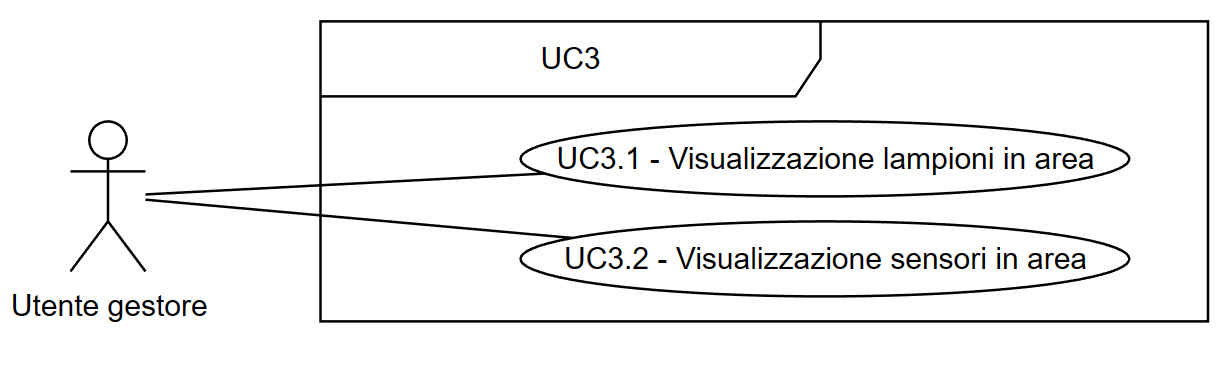
\includegraphics[width=\textwidth]{contenuti/img/casi_uso_grafici-uc3.png}
    \caption{Dettaglio dell'UC03}
    \label{fig:uc03}
\end{figure}

\subsection{UC03.1 Visualizzazione lampioni in area}
\paragraph{Intenzione in contesto} L'attore primario vuole vedere quali lampioni sono presenti in una determinata area.

\paragraph{Attore primario} L'attore primario è l'utente gestore.
\paragraph{Precondizioni}L'attore primario è riconosciuto ed autorizzato dal sistema.
\paragraph{Postcondizioni} L'attore primario visualizza quali lampioni sono presenti in una determinata area.

\paragraph{Scenario principale}
\begin{enumerate}
    \item L'utente richiede di visualizzare che lampioni siano in un'area;
    \item l'utente visualizza una lista dei lampioni in un'area.
\end{enumerate}

\subsection{UC03.2 Visualizzazione sensori in area}
\paragraph{Intenzione in contesto} L'attore primario vuole vedere quali sensori sono presenti in una determinata area.
\paragraph{Attore primario} L'attore primario è l'utente gestore.
\paragraph{Precondizioni}L'attore primario è riconosciuto ed autorizzato dal sistema.
\paragraph{Postcondizioni} L'attore primario visualizza quali sensori sono presenti in una determinata area.

\paragraph{Scenario principale}
\begin{enumerate}
    \item L'utente richiede di visualizzare che sensori siano in un'area;
    \item l'utente visualizza una lista dei sensori in un'area.
\end{enumerate}